% replace all text with your own text.
% in this template few examples are mention
\chapter{Methodology}
\label{ch:method} % Label for method chapter
Text Here

\section{Problem Description and Requirements}

The primary problem that the Tank Tactics project aims to address is the development of an online multiplayer tank battle game that overcomes the limitations of traditional multiplayer games, such as the need for manual port forwarding and IP address sharing. This task presents several challenges, including the need for seamless multiplayer connectivity, the creation of engaging gameplay mechanics, and the incorporation of advanced features to enhance the overall gaming experience.
\\
\noindent
\\
Developing an online multiplayer game like Tank Tactics requires a fast and efficient networking solution. The game must support multiple players interacting in real-time, which necessitates a secure, efficient, and low-level latency network. Any delay or lag in the game can significantly impact the user experience, making seamless networking crucial for the success of the project.
\\
\noindent
\\
Another significant challenge is the creation of engaging gameplay mechanics. Tank Tactics should feature intuitive tank controls, precise shooting mechanics, and a dynamic coin collection system. These core gameplay elements must be designed to provide an enjoyable and engaging experience for players.
\\
\noindent
\\
The incorporation of advanced features is also a key requirement for Tank Tactics. The game should include elements such as a real-time leaderboard, mini-map, healing zones, and bounty coins to add depth and variety to the gameplay. The specific context of the project also plays a vital role. Tank Tactics is designed to cater to fans of .io-style games and classic tank-based titles. The game should draw inspiration from these genres to create a familiar and intuitive experience for players. The target platform for the game is the Unity game engine, which influences the development process and the choice of networking technologies.
\\
\noindent
\\
Moving on to the requirements of the project, the functional requirements include seamless multiplayer connectivity, engaging gameplay mechanics, and the incorporation of advanced features. Seamless multiplayer connectivity is essential for allowing up to 20 players to interact in the same game environment without the need for manual port forwarding or IP address sharing. Engaging gameplay mechanics, such as intuitive tank controls and precise shooting are necessary and advanced features, like leaderboards, and mini-maps enhance the overall gaming experience.
\\
\noindent
\\
The non-functional requirements of the project include performance optimisation accessibility, and scalability. Performance optimisation is crucial for maintaining a smooth and responsive gaming experience for all players, even as the number of concurrent users increases. The game should also be accessible, with a user-friendly interface and minimal technical barriers to entry.
\\
\noindent
\\
In summary, the development of Tank Tactics presents several challenges and requirements that need to be addressed. The aim is to create an engaging, competitive, and accessible online multiplayer tank battle game by leveraging the power of Unity's multiplayer technologies and carefully considering these factors. 

\section{Technologies}
This section explores deeper into the key technologies employed in the development of Tank Tactics, providing a comprehensive overview of the Unity game engine, Visual Studio, C\# programming language, Unity Netcode, and Unity Gaming Services. By leveraging these powerful tools and frameworks, the project aims to create a seamless, engaging, and accessible online multiplayer gaming experience that effectively addresses the challenges and requirements outlined in section 3.1.

\subsection{Unity Game Engine}

Unity, as discussed in Chapter 2 (section 2.4.1), is a widely adopted cross-platform game engine that offers an extensive set of tools and features for game development. Its user-friendliness, versatility, and support for both 2D and 3D games across multiple platforms make it an ideal choice for the Tank Tactics project.
\\
\noindent
\\
One of the key advantages of using Unity for Tank Tactics is its component-based architecture and modular approach to game object composition. This design philosophy simplifies the development process and promotes code reusability by allowing developers to create and modify individual components without affecting the entire game object. This modular approach enables the Tank Tactics project to be efficiently created and iterate on gameplay mechanics, visual assets, and multiplayer functionality, streamlining the development workflow and reducing the time required to implement new features or make changes to existing ones.
\\
\noindent
\\
The Unity editor's intuitive interface and customisable layout further enhance the development experience. The editor provides a wide range of built-in tools for scene editing, asset management, and debugging, allowing developers to work more efficiently and effectively. For example, the scene view enables developers to visually design and manipulate game objects, while the hierarchy window provides a clear overview of the game object structure. The inspector window allows developers to modify the properties and components of selected game objects, and the project window serves as a central hub for managing and organizing game assets.
\\
\noindent
\\
In addition to these core features, Unity offers a vast ecosystem of plugins, extensions, and asset packages through the Unity Asset Store. These resources can significantly accelerate the development process by providing pre-built solutions, art assets, and tools that can be easily integrated into the project. Tank Tactics project can leverage these assets to enhance the game's visual quality, implement complex gameplay mechanics, or extend the functionality of the Unity editor to suit the project's specific needs.
\\
\noindent
\\
By leveraging the power and flexibility of the Unity game engine, the Tank Tactics project can benefit from a streamlined development process, a modular and reusable codebase, and a rich ecosystem of tools and assets. These advantages ultimately contribute to the creation of a polished, engaging, and accessible multiplayer gaming experience.

\subsection{Visual Studio and C\#}

Unity's primary scripting language is C\#, a powerful and versatile object-oriented programming language that is well-suited for game development. To write and debug C\# scripts efficiently, Visual Studio, a feature-rich integrated development environment (IDE), is the recommended choice for Unity projects.
\\
\noindent
\\
Visual Studio offers a wide range of productivity-enhancing features that streamline the coding process and help developers write clean, efficient, and maintainable code. One of the most notable features is IntelliSense, an intelligent code completion system that provides real-time suggestions and auto-completion for variables, methods, and classes as developers type. This feature significantly reduces the time required to write code and minimizes the risk of syntax errors, allowing developers to focus on implementing gameplay logic and mechanics.
\\
\noindent
\\
In addition to IntelliSense, Visual Studio provides real-time error detection and highlighting, which helps developers identify and resolve issues quickly. The IDE continuously analyzes the code as it is written, underlining potential errors and offering suggestions for fixes. This feature is particularly valuable in a complex project like Tank Tactics, where maintaining code quality and minimizing bugs is crucial for a smooth and enjoyable multiplayer experience.
\\
\noindent
\\
Visual Studio also offers powerful debugging tools that allow developers to investigate and resolve issues in their code. The debugger enables developers to pause the execution of the game at specific points, inspect variable values, and step through the code line by line to identify the source of problems. The IDE also provides advanced debugging features, such as conditional breakpoints and the ability to modify variable values during runtime, which can be invaluable when troubleshooting complex gameplay mechanics or multiplayer interactions.
\\
\noindent
\\
C\#'s object-oriented nature and extensive class library make it an ideal language for implementing intricate gameplay mechanics, and multiplayer network logic. The language supports essential object-oriented programming concepts, such as encapsulation, inheritance, and polymorphism, which allow developers to create modular, reusable, and maintainable code structures. By leveraging these features, the Tank Tactics project can be made with a codebase that is easy to understand, modify, and extend throughout the development process.
\\
\noindent
\\
Furthermore, C\# offers a wide range of built-in classes and libraries that simplify common programming tasks, such as string manipulation, file I/O, and collections. The language also provides support for advanced features like LINQ (Language Integrated Query), which enables developers to write expressive and concise queries for data manipulation and filtering. These features can significantly reduce the amount of boilerplate code required and allow developers to focus on implementing game-specific logic.
\\
\noindent
\\
By utilizing C\# and Visual Studio, the Tank Tactics project can benefit from a robust and efficient development environment that promotes code quality, maintainability, and extensibility. The combination of a powerful programming language and a feature-rich IDE empowers developers to create engaging gameplay mechanics, optimize performance, and ensure a smooth and enjoyable multiplayer experience for players.

\subsection{Unity Netcode and Unity Gaming Service}

Tank Tactics makes use of Unity's Netcode for GameObjects (NGO) framework and Unity Gaming Services (UGS) Relay \& Lobby to solve the multiplayer connectivity issues mentioned in Chapter 1 (section 1.2) and Chapter 2 (section 2.2).
\\
\noindent
\\
Unity Netcode for GameObjects (NGO) is a high-level networking library that abstracts the complexities of low-level network communication, allowing developers to focus on creating gameplay logic and synchronizing objects across the network. NGO is built on top of the Unity Transport Package, a low-level networking library that manages connections using UDP (User Datagram Protocol) and handles reliable and unreliable message sending.
\\
\noindent
\\
One of the key advantages of using NGO in Tank Tactics is its simplicity and ease of use. The framework provides a set of components and APIs that seamlessly integrate with Unity's existing GameObject and component system, making it easier for developers to add multiplayer functionality to their games. For example, the NetworkManager component acts as the core orchestrator for multiplayer sessions, handling tasks such as server startup, client connection, and scene management. The NetworkBehaviour component, on the other hand, enables developers to define which game objects and properties should be synchronized across the network.
\\
\noindent
\\
NGO also provides a range of built-in features that simplify common multiplayer tasks. These include object spawning, state synchronization, and remote procedure calls (RPCs). Object spawning allows the server to create game objects on all connected clients, ensuring that all players see the same objects in the game world. State synchronization keeps the game state consistent across all clients by automatically sending updates for synchronized variables whenever their values change. RPCs enable developers to define methods that can be invoked remotely by other clients or the server, facilitating communication and interaction between players.
\\
\noindent
\\
To further enhance the multiplayer experience and address the challenges associated with manual port forwarding and IP address sharing, Tank Tactics integrates Unity Gaming Services (UGS) Relay \& Lobby. UGS Relay is a managed service that provides a secure and scalable infrastructure for hosting multiplayer game sessions. By leveraging the Relay service, Tank Tactics can establish connections between players without requiring them to configure their routers or firewalls, eliminating the need for manual port forwarding and ensuring a seamless and accessible multiplayer experience.
\\
\noindent
\\
UGS Lobby, on the other hand, offers a convenient way for players to find and join multiplayer game sessions. The Lobby service allows developers to create and manage game lobbies programmatically, enabling players to browse available sessions, join existing lobbies, or create new ones. This feature streamlines the matchmaking process and provides a centralized hub for players to connect and interact with each other before starting a game.
\\
\noindent
\\
The combination of Unity Netcode for GameObjects and Unity Gaming Services Relay \& Lobby enables Tank Tactics to implement a client-hosted listen server model, as described in Chapter 2 (section 2.3.5). In this hybrid network topology, one of the players acts as both a client and a server, hosting the game for other players who connect as clients. This approach offers several benefits, such as reduced hosting costs and improved accessibility, while still maintaining the advantages of a client-server architecture, such as better security and simplified game state management. By utilising the power of Unity Netcode and Unity Gaming Services, Tank Tactics can deliver a smooth, responsive, and seamless multiplayer experience that effectively addresses the challenges associated with traditional multiplayer game development. These technologies align with the project's objectives, as outlined in Chapter 1 (section 1.3), and provide a robust foundation for implementing the game's core multiplayer features and mechanics.

\section{Implementations}
This section provides a comprehensive overview of the implementation of Tank Tactics, covering various aspects such as game design, project setup, core gameplay mechanics, multiplayer architecture, and UI/game management.

\subsection{Game Design}
Tank Tactics is designed as an engaging, combat multiplayer tank battle game. The core gameplay resolves around players controlling tanks, collecting coins, and using the designated healing zones around the map, killing other players to collect bounty coins that are dropped. The game incorporates various other features to enhance the overall experience, including a real-time leaderboard, and a mini-map.
\\
\noindent
\\
The game design aims to provide an enjoyable experience for up to 20 players simultaneously. It draws inspiration from popular .io style games and classic tank-based titles.

\subsection{Project Setup}
Tank Tactics is developed using the Unity game engine, taking advantage of its extensive features and tools for game development. The project is structured in a modular and organized manner, with various scripts, prefabs, and assets carefully categorized based on their functionality. This approach ensures maintainability, ease of debugging, and flexibility for future expansion.
\\
\noindent
\\
The scripts are categorized into different functionalities, such as core player mechanics, combat systems, coin management, networking, and UI/game management. This modular approach allows for easy maintenance, debugging, and expansion of the game's features.

\subsection{Core Gameplay Mechanics}
The core gameplay mechanics of Tank Tactics are implemented through various scripts that handle different aspects of player functionality, combat, coin management, and game events. The tank movement and aiming mechanisms are designed to be intuitive and responsive, allowing players to navigate the game world and engage in combat effectively. The shooting mechanics are fine-tuned to ensure a satisfying and balanced gameplay experience.
\\

\begin{figure}[h]
    \centering
    \begin{minipage}{0.49\textwidth}
    \centering
    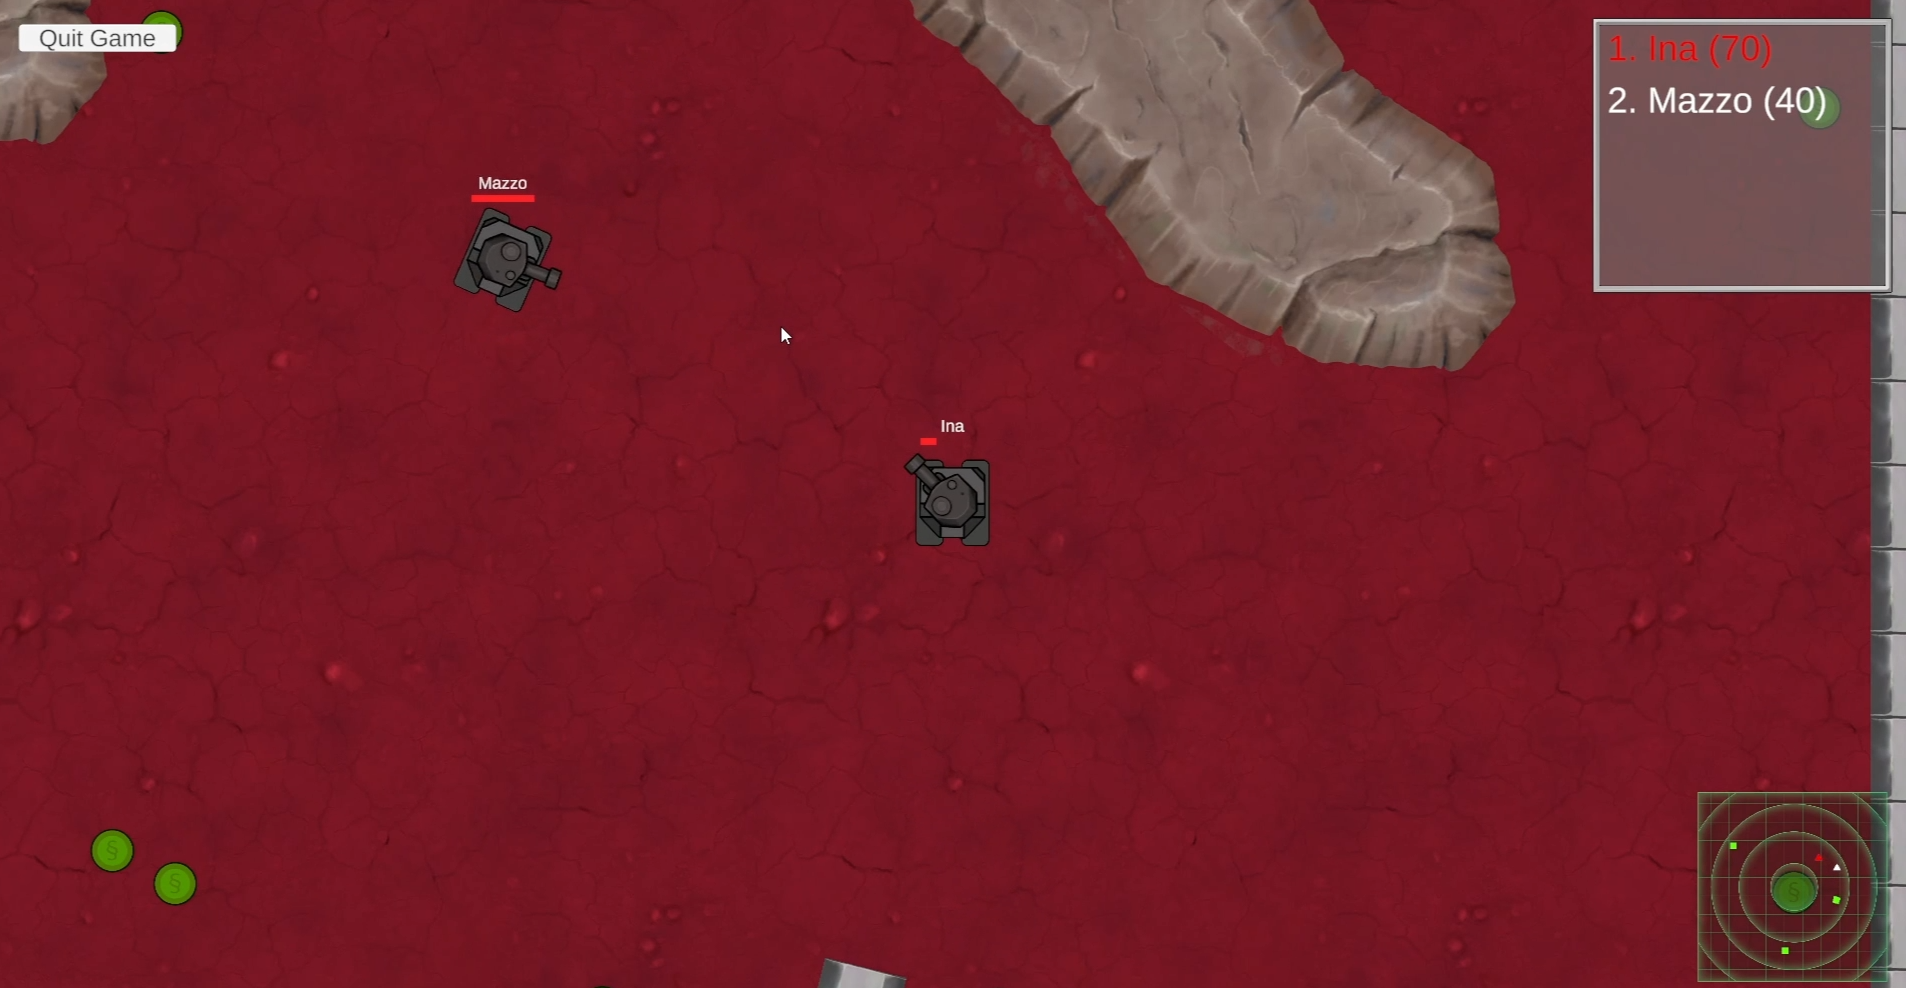
\includegraphics[width=1\textwidth]{figures/GamePlay.png}
    \caption{Gameplay}
    \label{fig:player_gameplay}
    \end{minipage}
\end{figure}

\noindent The game features a coin collection system, where players can gather coins scattered throughout the map. These coins serve as a form of in-game ammo and currency, enabling players to utilise the designated healing zones and enhance their gameplay. The coin management system keeps track of each player's coin balance and handles the spawning and collection of coins seamlessly.
\\
\noindent
\\
Combat mechanics, such as damage calculation and health management, are implemented to create a challenging and rewarding experience. Players can engage in battles with other tanks, with the outcome determined by factors such as weapon accuracy, damage output, and strategic positioning. Healing zones and player respawning mechanics add an extra layer of strategy and ensure fair gameplay.

\subsection{Network Architecture}
Tank Tactics employs a client-hosted listen server model, which combines elements of client-server and peer-to-peer architectures. This approach allows for efficient network communication and synchronization between players while minimizing the need for dedicated server infrastructure.
\\
\noindent
\\
The game leverages Unity's Netcode for GameObjects (NGO) framework to handle the underlying network communication and synchronization. NGO simplifies the process of implementing multiplayer functionality by providing a high-level API for managing network objects, synchronizing game states, and handling client-server interactions.
\\
\noindent
\\
To enhance the multiplayer experience further, Tank Tactics integrates Unity Gaming Services (UGS). UGS provides a suite of tools and services for features such as player authentication, matchmaking, and lobby management. By leveraging UGS, the game ensures a seamless and user-friendly multiplayer experience, allowing players to easily connect, join games, and interact with each other.
\\

\begin{figure}[h]
    \centering
    \begin{minipage}{0.49\textwidth}
    \centering
    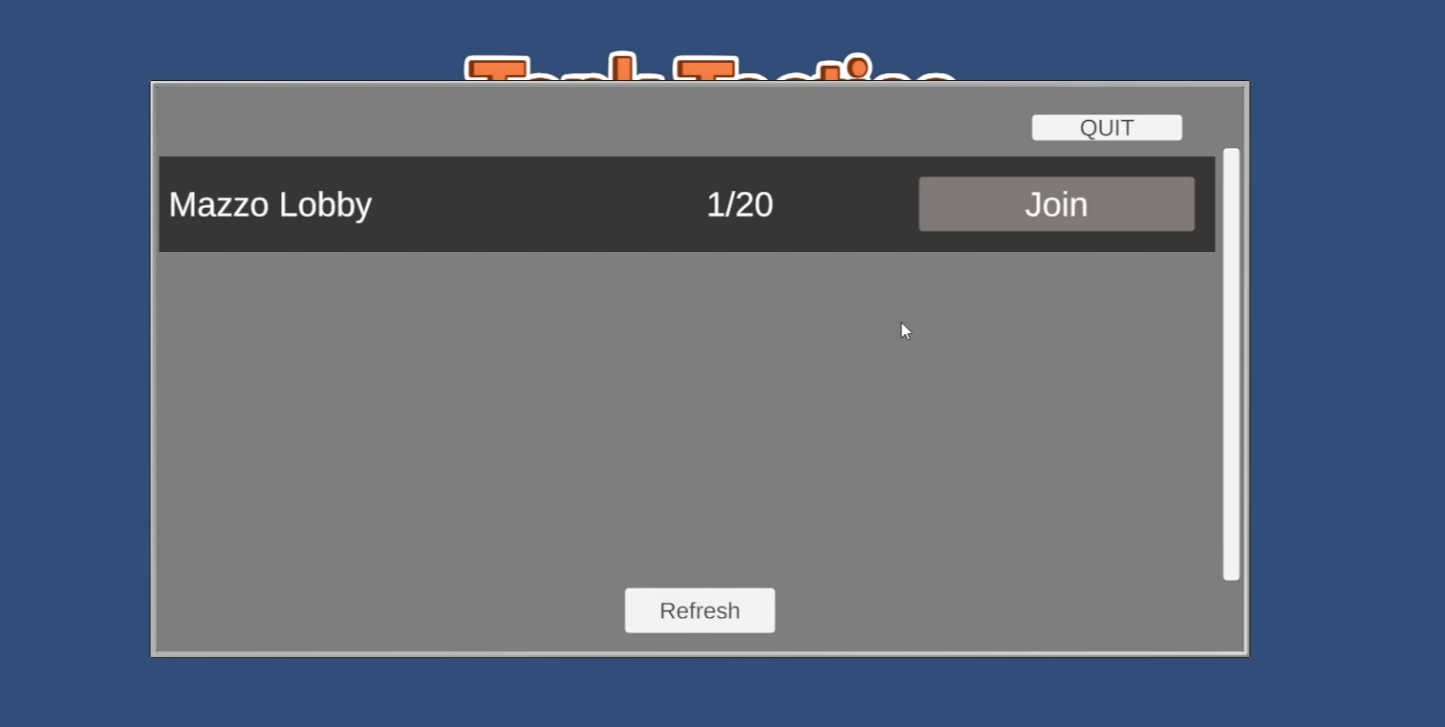
\includegraphics[width=1\textwidth]{figures/Lobby.png}
    \caption{Player Lobby}
    \label{fig:player_lobby}
    \end{minipage}
\end{figure}

\noindent The multiplayer architecture is designed to handle various aspects of network communication efficiently, such as object spawning and despawning, position synchronization, and event propagation. The implementation ensures a smooth and responsive gameplay experience, minimizing the impact of network latency and optimizing bandwidth usage.

\subsection{UI and Game Management}
The user interface (UI) and game management aspects of Tank Tactics are implemented to provide players with a polished and intuitive experience. The UI is designed to be clean, informative, and easy to navigate, allowing players to access essential information and perform actions effortlessly.
\\
\noindent
\\
Players can browse available lobbies, create their own lobbies, and join existing ones. The lobby management system handles player connections, disconnections, and game session initialization.
\begin{figure}[h]
    \centering
    \begin{minipage}{0.49\textwidth}
    \centering
    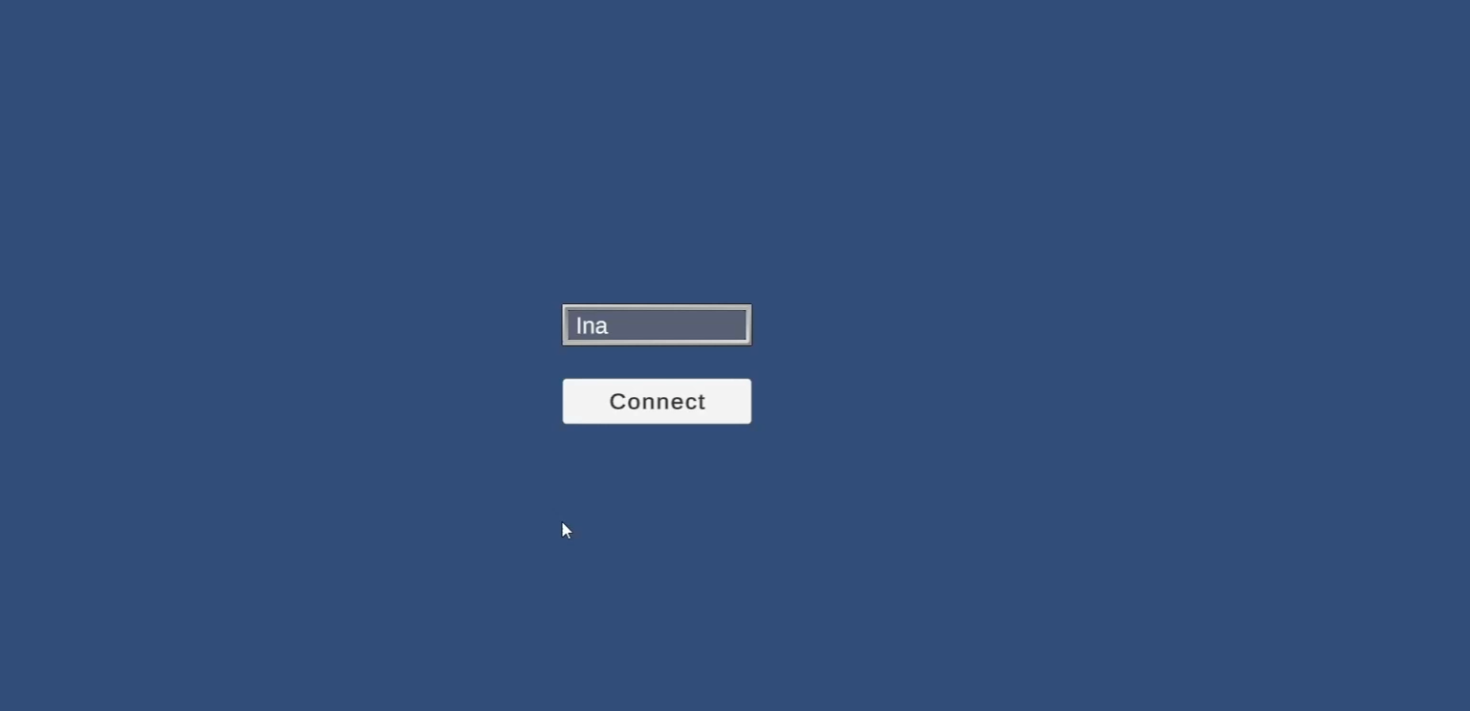
\includegraphics[width=1\textwidth]{figures/Connection.png}
    \caption{Player Connection}
    \label{fig:player_connection}
    \end{minipage}
    \hfill
    \begin{minipage}{0.49\textwidth}
    \centering
    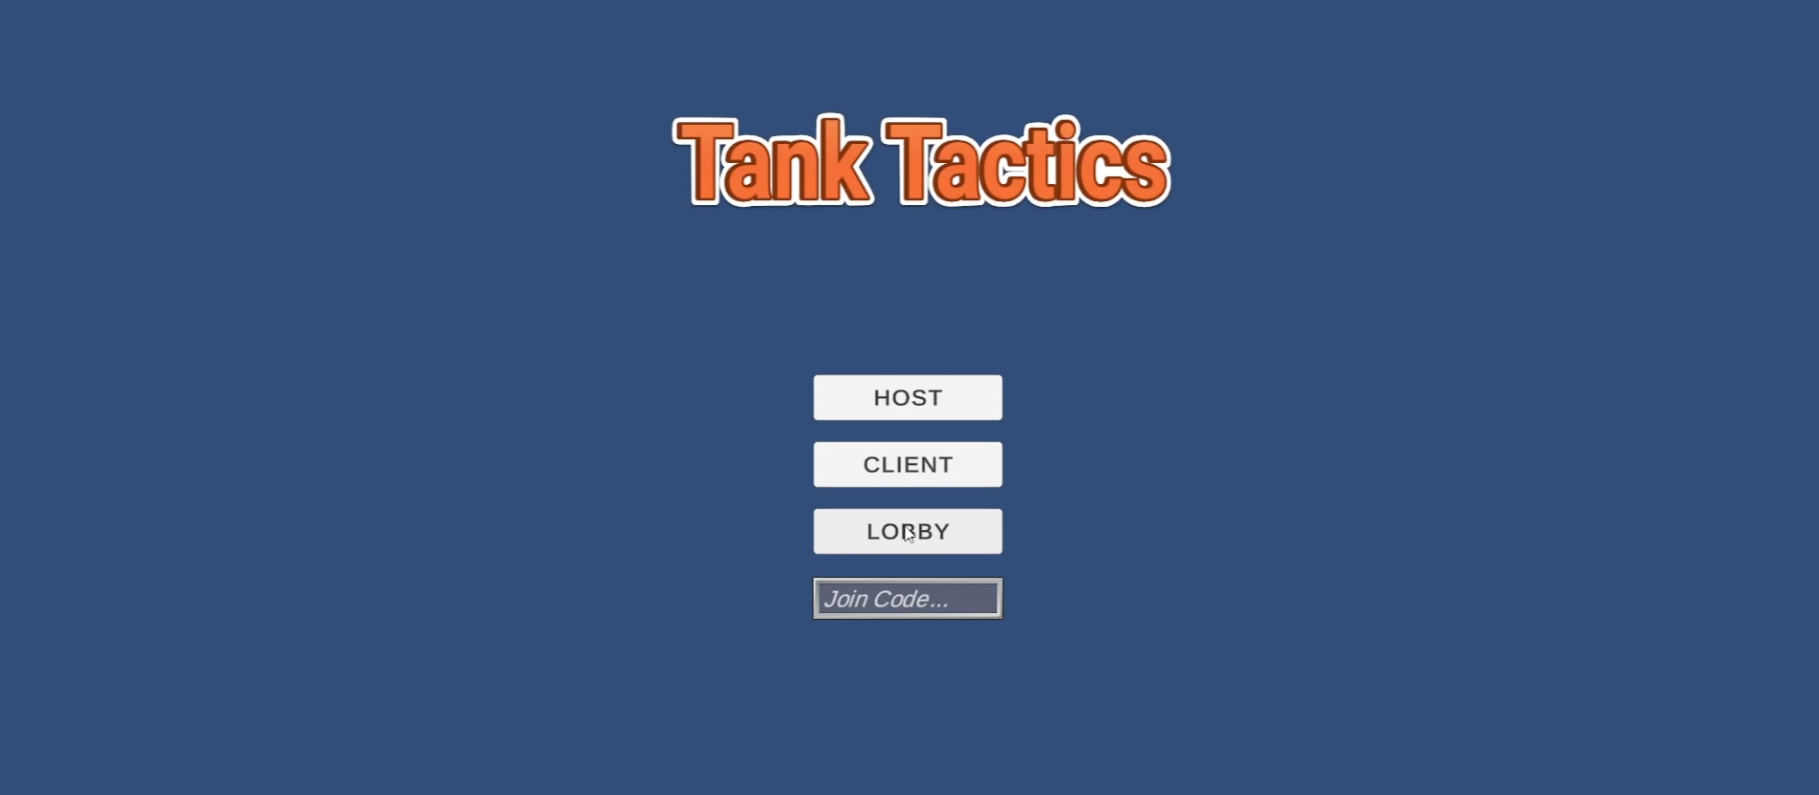
\includegraphics[width=1\textwidth]{figures/MENU.png}
    \caption{Menu Screen}
    \label{fig:player_menu}
    \end{minipage}
\end{figure}
\\
\\
\\
Game management scripts handle various aspects of the game's flow and progression. This includes managing game states, triggering events, and handling player actions. The implementation ensures a consistent and synchronized experience for all players, regardless of their role as a host or client.
\\
\noindent
\\
Overall, the UI and game management components of Tank Tactics are designed to enhance the player experience, providing a seamless and intuitive interface for navigating the game world, managing multiplayer sessions, and interacting with other players.
%\clearpage %  use command \clearpage when you want section or text to appear in the next page.


\section{Summary}
In summary, the implementation of Tank Tactics showcases a modular and well-structured approach to game development. The game design prioritizes player engagement, and competition, while the project setup ensures maintainability and extensibility. The core gameplay mechanics are implemented to provide a dynamic and rewarding experience, with smooth tank controls, strategic coin collection, and intense combat. The multiplayer architecture leverages Unity's NGO framework and UGS to enable efficient network communication and a seamless multiplayer experience. The UI and game management aspects are designed to be intuitive, informative, and user-friendly, enhancing the overall player experience. By combining these elements, Tank Tactics delivers an immersive and exciting multiplayer tank battle game that encourages, strategy, and skill.

